\chapter{Introduction}

As the scale of enterprise web applications grows rapidly, finding an effective way for testing site reliability is becoming increasingly important. As a widely-used testing technique, penetration testing is able to exploit the vulnerabilities of a web application back-end by simulating sending HTTP requests from the client side. Since penetration testing is used to test as many parts of an application as possible, comprehensiveness is the most important factor in performing penetration testing. An ideal penetration test is the one that generates HTTP requests which cover 100\% of the server-side code.

Traditionally, penetration tests are performed as black-box testing, which views the program to be tested as a "black box" whose implementation detail is unknown to the tester. Black-box testing allows the tester to focus on only the input and the output generated by the program; however, since the inner functionality of the program is unknown, it is difficult for the tester to generate a comprehensive test suite that guarantees 100\% back-end code coverage. In traditional manual penetration testing, a tester could only apply "educated guesses" when creating test requests. Some recent research proposed automated penetration testing using AI techniques such as genetic algorithm \cite{ref1} and neural network models \cite{ref2}. Although these automated approaches showed promising results in some scenarios, by nature they are still black-box testing, only improving the accuracy of "educated guess" by inferring from the statistical analysis results generated from the differences between expected outputs and actual outputs.

The lack of comprehensiveness and efficiency in black-box penetration testing prompted us to propose a new approach that performs white-box testing, during which tests are performed by looking at the implementation details in the source code of the program itself. In our implementation, both the interfaces that an application exposes and all the request data that is processed in the back-end can be inferred from static analysis results. The test suite goes through the program and checks at what positions each HTTP request variable is used. If some other variables are involved at any of the positions, then the program will use the result of data flow analysis to construct the exact value for such variables, which are also the possible values that the HTTP request variable could take. The test suite uses a library developed by Christensen, Møller, and Schwartzbach \cite{ref4} to construct an automaton that represents possible string values during string variable construction.

As another major part of penetration testing, interface discovering was traditionally done by doing web crawling. However, since modern web frontend is becoming increasingly dynamic, only extracting information from the client-side HTML pages does not guarantee enough interfaces are discovered. In 2007, Halfond and Orso \cite{ref3} proposed a novel approach for discovering web application interfaces using static analysis. Such technique showed promising results for finding and grouping dynamic interfaces that are not exposed directly by the front-end.
In this project, the same algorithms proposed by Halfond et al. is applied for doing interfaces discovery, but is targeted for PHP web applications.


%% This is a figure
% \begin{figure}
% 	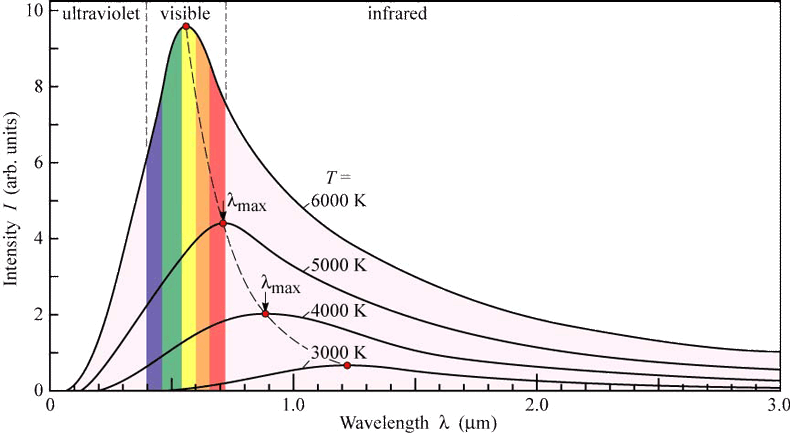
\includegraphics[width=\textwidth]{figures/exampleFigure.png}
% 	\caption{This is an example Figure.}
% 	\label{Figure in Chapter 1}
% \end{figure}

%% This is a table
% \begin{table}
% \caption{This is an example Table.}
% \begin{center}
% \begin{tabular}{ccc}
% x & f(x) & g(x) \\
% \hline
% 1 & 6 & 4  \\
% 2 & 6 & 3  \\
% 3 & 6 & 2  \\
% 4 & 6 & 2  \\
% \label{Table in Chapter 1}
% \end{tabular}
% \end{center}
% \end{table}
